\documentclass[output=paper]{langscibook}
\ChapterDOI{10.5281/zenodo.5578826}

%This is where you put the authors and their affiliations
\author{Stephen Dettweiler\affiliation{SIL International}}

%Insert your title here
\title{Subordinate clauses in Dadiya: Field research on the use of enclitic -I}  
\abstract{The author, Stephen Dettweiler, is a member of SIL International. From 1991 to 2017 he lived in Nigeria doing research on Nigerian languages. He currently functions as a remotely based linguistics consultant available to Nigerian language projects. The Dadiya project recently requested his assistance to investigate the use of a clitic -I, observed to occur frequently at the end of subordinate clauses in narrative and hortatory texts. This article shows how widespread the enclitic is for various types of subordinate clauses in three Dadiya narratives, accounting for its presence (and occasional absence) in both simple and nested clause structures.}

\begin{document}
\SetupAffiliations{mark style=none}
\maketitle

\section{Introduction}

Dadiya [dbd]\footnote{Dadiya is spoken in the area of northeastern Nigeria where Gombe, Taraba and Adamawa State boundaries meet. Its classification in the Ethnologue \citep{EberhardFennig2019} is Niger-Congo, Adamawa family, Waja-Jen group.} is an Adamawa language spoken in northeastern Nigeria. A notable feature of most Dadiya subordinate clauses is the use of the harmonizing enclitic -I (realized as /i/ or /ɪ/ depending on the [ATR] value of the immediately preceding vowel) in clause-final position.\footnote{In general, the enclitic harmonizes with the vowel(s) of the word it follows, i.e. its host. Though this paper shows many examples of clitic-host harmony, apparent examples of disharmony were investigated by my SIL colleague, Coleen Starwalt. She discovered that there was no disharmony, but inconsistency in representing the clitic vowel due to orthographic convention. Appendix A shows a chart of the vowels and how they are represented in the orthography.}

The Dadiya proverb below, comparing a dog and a lion, is an example. Both of the animals are described using a relative clause, and both relative clauses begin with a connective and end with the -I clitic. The subordinate clauses are bracketed in all lines.

\ea
\gll səgan [nɨ nən dʊʊm-ɨ] a laa tulum [nɨ a bula bula-i]\\
dog [\textsc{rel} be.with life-??] 3s.\textsc{pfv} surpass lion [\textsc{rel} 3s.\textsc{pfv} die die-??]\\
\glt `A dog [which has life] is better than a lion [which is dead].'
\z

Work on three Dadiya narrative texts has shown that the -I clitic is used at the close of almost every subordinate clause in natural narrative. But there are a few subordinate clauses that seem to lack the clitic marking, and sometimes a clause marked with the -I clitic appears to be a main clause. Also, the same clitic (or one remarkably like it) is found in a few other places that are phrase-final but not clause-final. What then is a comprehensive description of the distribution and functions of this clitic?

Dadiya is in vigorous use orally as the first language of over 70,000 people \citep{EberhardFennig2019}, but its linguistic features are under-documented. \citet{Jungraithmayr1968} includes a helpful six-page description of the Dadiya grammar and lexicon, \citet{Kleinewillinghofer1996} comments on it in connection with near relatives Tula and Waja, and also provides a 100-item wordlist of Dadiya alongside others in the Tula-Waja subgroup \citep{Kleinewillinghofer2014}. \figref{fig:dettweiler:DadiyaRelatives} shows Dadiya in the context of its closest Adamawa relatives as given by \citet{2019}. The number of languages in each subgrouping is given in parentheses. Most Adamawa languages are as sparsely documented as Dadiya is. \figref{fig:dettweiler:NigeriaLanguages} shows the geographic placement of the Adamawa family of languages within Nigeria, alongside other major language families (adapted with permission from \citealt[45]{Blench2007}).

\begin{figure}
% %     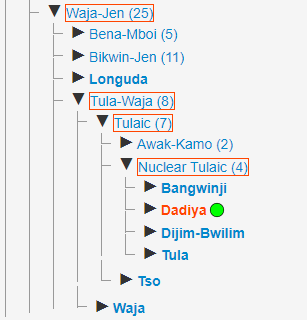
\includegraphics{figures/Dadiya.png}
    \begin{forest}for tree = {folder, grow'=0}
      [Waja-Jen
       [Bena-Mboi]
       [Bikwin-Jen]
       [Longuda
         [Tula-Waja
           [Tulaic
             [Awak-Kamo]
             [Nuclear-Tulaic
               [Bangwinji]
               [\textbf{Dadiya}]
               [Dijim-Bwilim]
               [Tula]
             ]
             [Tso]
           ]
           [Waja]
         ]
       ]
      ]
    \end{forest}
    \caption{The Dadiya Language and its close Adamawa relatives}
    \label{fig:dettweiler:DadiyaRelatives}
\end{figure}

\begin{figure}
    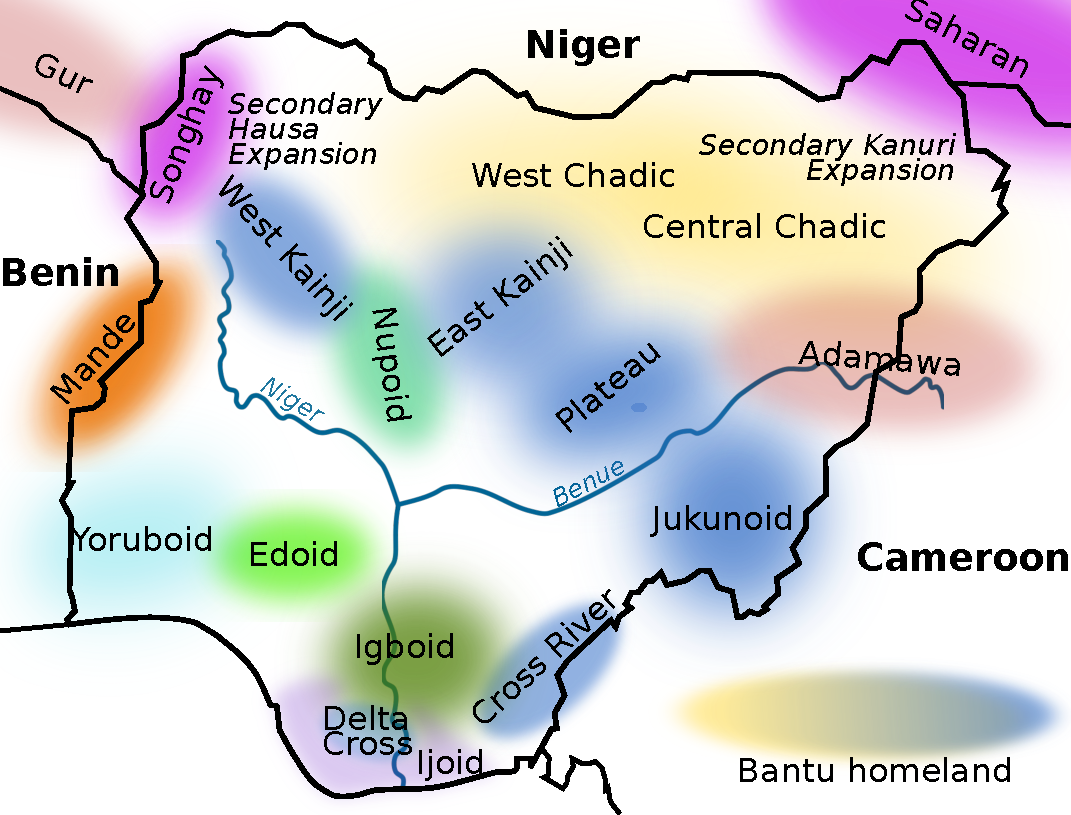
\includegraphics[width=.8\textwidth]{figures/nigeria.pdf}
    \caption{The Nigeria context of the Adamawa language family}
    \label{fig:dettweiler:NigeriaLanguages}
\end{figure}

\section{Methods}

SIL translation consultant Randy Groff has worked with the Dadiya language project team since 2005. His work with them has provided the impetus for this study. Since 2013 they have collected a number of verb paradigms and a series of three narrative texts which they later entered in Fieldworks Language Explorer. These materials, particularly the narratives, were intended for the exploration of Dadiya sentence structure and verbal morphology in natural text. After discussions with Mr. Groff in early 2017, I agreed to make careful analysis of the three narratives a high priority.

\begin{sloppypar}
The widespread use of a clitic in marking the end of Dadiya subordinate clauses had already been identified as an important focal point for the analysis of narrative structure. In the newly revised Dadiya orthography \citep{Committee2018}, this enclitic is written as a suffix -i or -ɨ on the word which it follows. Commonly\footnote{The use of two other segmentally identical morphemes is discussed at the end of \sectref{sec:dettweiler:3}.} this suffix signals the end of a clause which is subordinate to (dependent on) a main clause nearby, so that this usage has been glossed as DEP in the three narrative texts. In the body of this paper, this enclitic is often referred to as the -I clitic as a concise way to summarize its two forms.\footnote{The orthographic forms 〈i〉 and 〈ɨ〉 have been chosen to represent the Dadiya vowels [+ATR] /i/ and [\textminus ATR] /ɪ/ respectively. Because of its two forms, called allomorphs, the enclitic in focus can be represented as a morphophoneme /-I/. This enclitic always harmonizes with the last vowel in the preceding word.} The Dadiya line given for each sentence example uses the current orthography throughout, except that the separation of affixes and clitics may be shown using – and = respectively, symbols which are not in the orthography.
\end{sloppypar}

Prior to my investigation, two of the three Dadiya narratives had been completely interlinearized using Fieldworks Language Explorer \citep{SILInternational2019a}. In addition to completing the interlinearization of the third narrative, I used the Fieldworks software to prepare clause constituent structure charts for all three. The three narratives are listed here in the order studied. A thematic Dadiya word from each narrative is given in uppercase as its title (with gloss italicized in the English title):

\begin{enumerate}\sloppy
    \item TAAL (A Story which Gives \textit{Fear}) – autobiographical narrative, 28 sentences in 6 paragraphs, told by Joseph Goje.
    \item DOLA (They Sat \textit{Courtship} Together) – 3rd-person human interest story, 20 sentences in 3 paragraphs, told by Iliya Dokan.
    \item KƗLAN (Why I Stopped \textit{Fighting}) – autobiographical narrative, 41 sentences in 4 paragraphs, told by Jothan Joel.
\end{enumerate}

\noindent Using sentence 16 of the TAAL narrative, \figref{fig:dettweiler:StructureChart} illustrates how the phrases and clauses of a sentence are separated into the pre-nuclear, core (or nuclear) and post-nuclear columns of a chart. Patterns of morphology, syntax, and discourse structure are revealed as the analyst notes differences and similarities between the various columns. From \figref{fig:dettweiler:StructureChart} a question arises concerning the two dependent clauses 16b and 16c (both relative, with \textit{kaa jəl} `certain thing' as head): why is there only one occurrence of the -I clitic in this post-nuclear part of Sentence 16 when there are two dependent clauses?

\begin{figure}
    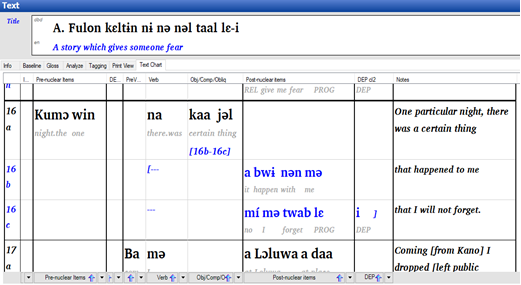
\includegraphics[width=\textwidth]{figures/Structure.png}
    \caption{Constituent structure chart for TAAL16}
    \label{fig:dettweiler:StructureChart}
\end{figure}

For twenty-one hours of consultation spread over ten days, the Dadiya project team and I along with translation consultant Randy Groff went through the TAAL and DOLA narratives sentence by sentence. The main technique used was to encourage Dadiya speakers to unpack the meanings (both semantics and pragmatics) of various sentences and clauses to help reveal the forms, syntax, and discourse structure. Often I asked questions based on observations I had made during the preparatory sentence-by-sentence charting using Fieldworks. This method solidified our grasp of the structure and meaning of the narratives and enhanced our understanding of Dadiya grammar as revealed in the text.  The third narrative, KƗLAN, had been glossed prior to the consultation but no free translation had been supplied. This made it difficult to prepare clause constituent charts for KƗLAN in advance of the consultation. However, using consultation time to go through the narrative sentence by sentence yielded an improved understanding of what underlay the forms of the text as well as an accurate free translation for each sentence.

\section{Types of subordinate clauses}\label{sec:dettweiler:3}\largerpage

\subsection{General remarks}

Dadiya has the three major types of subordinate clauses which are found in nearly all the world's languages. A relative clause functions as modifier of a noun phrase; an adverbial clause modifies a verb phrase or an entire proposition; a complement clause functions as a ``sentential expansion" of the subject or object slot of the sentence in which it is embedded \citep[374]{Longacre2007}. 

This section gives numerous Dadiya examples, drawn from the repertory of relative clauses, adverbial clauses, and complement clauses discovered in a study of the three narratives. It points out that all three types of Dadiya subordinate clauses close with the presence of the -I clitic in most cases, and investigates situations in which the clitic is absent. Finally, it  considers examples of morphemes that may be confused with the -I clitic.

\subsection{Relative clauses}

Dadiya makes frequent use of relative clauses. These function as nominal modifiers, subordinating a proposition which identifies or describes the referent called the head of the relative clause. For example, in the noun phrase \textit{children who are playing}, the relative clause \textit{who are playing} modifies the head noun, \textit{children}. The relativizer is the pronoun \textit{who}. In the noun phrase \textit{the children you thanked}, the head NP is \textit{the children} and there is no relativizer present (though any of the pronouns whom, who, or that could be used immediately after the head NP). A fruitful question to ask about a language is which grammatical relations it allows to be relativized \citep[326]{Payne1997}, so for Dadiya we particularly want to observe what grammatical roles the referent (indicated by the head NP) can take in the relative clause. The head also has a grammatical role in the sentence in which the relative clause is embedded, known as the matrix clause.

Each Dadiya relative clause presented here uses the -I clitic in one of its forms, 〈i〉 or 〈ɨ〉, as its final morpheme. Also, every Dadiya relative clause observed is a \textit{restrictive} or defining relative clause: this means it specifies or delimits the role of its referent in the situation described by the relative clause \citep[206]{Andrews2007}. The relative clause frequently begins with the relativizer \textit{nɨ}, glossed REL in examples \REF{ex:dettweiler:TAAL2}, \REF{ex:dettweiler:TAAL17} and \REF{ex:dettweiler:TAAL26}, but this morpheme is not obligatory,\footnote{Other examples will show that the morpheme \textit{nɨ} sometimes functions as a proximal demonstrative `this'. It is not unusual cross-linguistically to have several related functions for a single grammatical morpheme. For example, the Dadiya distal demonstrative \textit{gɔ} `that' also functions as a 3rd person singular object pronoun and as a complementizer. Grammatical structure usually makes it clear which function applies in each context.} as shown in example \REF{ex:dettweiler:DOLA3}. No difference has yet been noted between the verb forms in relative clauses compared to those of matrix clauses. Example \REF{ex:dettweiler:TAAL2} shows a relative clause that modifies the noun phrase \textit{fulon kɛltɨn} `story'. The kind of story specified by the relative clause is one which `gives a person fear'. In the matrix clause, this NP is object of the verb `give', but its role in the relative clause is as subject.

\ea Dadiya head NP \textit{fulon kɛltɨn} `story': object in matrix clause, subject of relative clause:
\label{ex:dettweiler:TAAL2} \\
\gll tuga mi gə nii fulon kɛltɨn [nɨ nə nəl taal lɛ =ɨ] \\
grandfather my 3s.\textsc{ipfv} give.me news talks [\textsc{rel} give heart fear \textsc{prog} =\textsc{dep}] \\
\glt `My grandfather would give me a story [that would frighten me (lit. be giving heart fear)].' TAAL2
\z

\noindent The matrix clause of \REF{ex:dettweiler:TAAL17} has \textit{daa} `place' as the location (marked with the preposition \textit{a}). The relative clause gives a name to this place, and its verb \textit{jou} `call' takes two objects. The first of these is the place referred to by the head NP and the second is the name, \textit{Dogon Dutse}. The first object slot is filled by a 3rd person singular pronoun \textit{gɔ} -- this is identified as a `trace' or \textit{resumptive} pronoun \citep[220]{Andrews2007}.

\ea Head NP \textit{daa} `place' is oblique in matrix clause, object of the relative clause:
\label{ex:dettweiler:TAAL17} \\
\gll Ba mə gəla ...a daa [nɨ jə jou lɛ gɔ Dogon Dutse =i] \\
coming 1s.\textsc{ipfv} drop ...\textsc{loc} place [\textsc{rel} 3p.\textsc{ipfv} call \textsc{prog} 3s.\textsc{obj} Dogon Dutse \textsc{dep}] \\
\glt `Coming I would drop ... at a place [that they are calling it Dogon Dutse].' TAAL17
\z

\noindent The relative clause of \REF{ex:dettweiler:DOLA3} has no REL at the beginning and the head NP functions in the relative clause as location. The subject of the relative clause \textit{gə} `she' refers to a highly topical participant in the DOLA narrative, the young woman with many suitors. The copula of location, \textit{wo} `be there', is most frequently observed in relative clauses (but see the response half of example \REF{ex:dettweiler:KƗLAN30}, where \textit{wo} occurs without the -I clitic).\largerpage

\ea Head NP \textit{daa} `place', use of copula \textit{wo}, no relativizer:
\label{ex:dettweiler:DOLA3} \\
\gll nəb-ɔ bɛ lɛ a daa [gə wo =i] \\
people-\textsc{def} come \textsc{prog} \textsc{loc} place [3s.\textsc{ipfv} be.there =\textsc{dep}] \\
\glt `The people were coming to the place [where she was].' DOLA3
\z

\noindent The evidence of \REF{ex:dettweiler:TAAL26} is that a relative clause can precede its matrix clause. This relative clause contains the topic of the story, information that is old to the audience. It is expected that a relative clause preceding its matrix clause would not contain new information.\footnote{The object pronoun \textit{gəm}, referring to a person (P), is distinct from the one in example \REF{ex:dettweiler:TAAL17} referring to a non-person. \citet[195--196]{Jungraithmayr1968} mentions such distinctions as a vestige of the Dadiya noun class system.}

\ea Object of the matrix clause is preposed head\,+\,RC, head is subject of the relative clause:
\label{ex:dettweiler:TAAL26} \\
\gll Jʊ [nɨ a bwɨ nən mə a gola =ɨ] mə kiyo gəm bɔ \\
thing [\textsc{rel} 3s.\textsc{pfv} happen with 1s.\textsc{obj} \textsc{loc} road =\textsc{dep}] 1s.\textsc{ipfv} tell 3s.\textsc{obj}.\textsc{p} not \\
\glt `The thing [that happened to me on the road], I didn't tell her.' TAAL26
\z

\subsection{Adverbial clauses}

Adverbial clauses ``attach to constructions that are already complete propositions" \citep[317]{Payne1997}, simply adding some information such as time, location, manner, or purpose to the proposition as an adjunct. So, unlike with relative clauses and complement clauses, there is no need to refer to a matrix clause in which the adverbial clause is embedded. The sentence in \REF{ex:dettweiler:TAAL10} shows a time clause which is subordinate to the following clause, and the enclitic is attached to the preceding word \textit{taal} `fear'.\footnote{In Dadiya orthography, this enclitic is always written as a suffix of the clause-final word, but I am referring to the phonological attachment which is shown by vowel harmonization.}

\ea Time clause (adverbial) marked with -I clitic:
\label{ex:dettweiler:TAAL10} \\
\gll Tɛtə mɨ a swɨ bɔ taal a bʊt-ɔ mɨ, [na n nyuwa taal =ɨ] a jəga i. \\
father my 3s.\textsc{pfv} like not fear on body-\textsc{def} my [when 1s.\textsc{pfv} hear fear =\textsc{dep}] 3s.\textsc{pfv} slap me \\
\glt `My father did not want fear in my body; [when I felt fear], he slapped me.' TAAL10
\z

\noindent The particle \textit{na} introduces the adverbial clauses in \REF{ex:dettweiler:TAAL10} and \REF{ex:dettweiler:KƗLAN4} and is glossed as a connective `if/when'. In these two sentences it introduces a condition or circumstance that qualifies the main clauses. In \REF{ex:dettweiler:KƗLAN4} it can be seen to act as a bridge between the first main clause and the second one.

\ea Condition clause bridging between two main clauses:
\label{ex:dettweiler:KƗLAN4} \\
\gll N bʊg nəl; [na ke bɔ ny =ɨ] nəl a bʊg i. \\
1s.\textsc{pfv} beat person; [if be.\textsc{neg} not thus =\textsc{dep}] person 3s.\textsc{pfv} beat me. \\
\glt `I would beat up on somebody, or (\textit{lit.} if it is not thus) somebody would beat up on me.' KƗLAN4
\z

\noindent Example \REF{ex:dettweiler:TAAL27} shows a purpose clause which follows the main clause it modifies. The main clause is in the imperfective (as shown by the pronoun and the use of progressive signified by the \textit{lɛ} particle) and the purpose clause, though having the same subject, is in the perfective aspect (as indicated by its subject pronoun).

\ea Purpose clause introduced without connective:
\label{ex:dettweiler:TAAL27} \\
\gll mí mə mwɨ lɛ [n yɔ nən {dɔm dɔm} =ɨ]. \\
not 1s.\textsc{ipfv} be.brave \textsc{prog} [1s.\textsc{pfv} go with closeness =\textsc{dep}] \\
\glt `I am not being brave [(so that) I go close].' TAAL27
\z

\subsection{Complement clauses}

A complement clause is a `notional sentence or predication' which functions as the subject or object of another `larger' predicate into which it is embedded \citep[52]{Noonan2007}. The larger predication is often called the matrix clause \citep[313]{Payne1997}. An example is the English sentence, \textit{I hoped that you would sell all the groundnuts}: the matrix clause is \textit{I hoped X} and the complement clause which is embedded in the matrix clause as its object is \textit{that you would sell all the groundnuts}.

A verb in the domain of thinking, feeling, or seeing (often called a cognitive verb) frequently takes a complement clause as its direct object. Examples \REF{ex:dettweiler:KƗLAN16}, \REF{ex:dettweiler:KƗLAN13} and \REF{ex:dettweiler:DOLA19} exemplify this, with verbs \textit{ko} `see', \textit{swɨ} `want', and \textit{nyəm} `know' respectively. The object complement clause for this kind of matrix verb can take a different subject from the matrix clause, as in \REF{ex:dettweiler:KƗLAN16} and \REF{ex:dettweiler:DOLA19}, or the same subject, as in \REF{ex:dettweiler:KƗLAN13}. Also, the verb of the complement clause is not reduced in its ability to be inflected from the verb of the matrix clause. All three complement clauses are marked with the DEP clitic.

\ea Cognitive matrix verb \textit{ko} `see':
\label{ex:dettweiler:KƗLAN16} \\
\gll mə ko [kaa bwɛ a jel a youl =i]. \\
1s.\textsc{ipfv} see [certain child 3s.\textsc{pfv} go.out at outside =\textsc{dep}]. \\
\glt `I saw [another child go outside].' KƗLAN16
\ex Cognitive matrix verb \textit{swɨ} `want':
\label{ex:dettweiler:KƗLAN13} \\
\gll a swɨ bɔ [a tʊm gən nən kwaan =ɨ] \\
3s.\textsc{pfv} want not [3s.\textsc{pfv} beat 3s.\textsc{obj}.\textsc{p} with power =\textsc{dep}] \\
\glt `He did not want [to beat him hard].' KƗLAN13
\ex Cognitive matrix verb \textit{nyəm} `know':
\label{ex:dettweiler:DOLA19} \\
\gll gə nyəm [jʊ bwɨ lɛ =ɨ]? \\
3s.\textsc{ipfv} know [thing happen \textsc{prog} =\textsc{dep}]? \\
\glt `Did she know [what was happening]?' DOLA19
\z

\noindent Other matrix verbs such as \textit{təl} `start' always have the same subject for matrix and complement clause, as in \REF{ex:dettweiler:DOLA12}, though the subject of the complement clause does not have to be explicit (cf. example \REF{ex:dettweiler:KƗLAN7}).

\ea Matrix verb \textit{təl} `start' with same subject in main and complement clauses:\label{ex:dettweiler:DOLA12}\\
\gll nəngɔ jə təl [jə yɨ dola-gɔ lɛ =ɨ]. \\
then 3p.\textsc{ipfv} start [3p.\textsc{ipfv} sit courting-\textsc{def} \textsc{prog} =\textsc{dep}]. \\
\glt `Then they started [courting (\textit{lit.} they were sitting the courting)].' DOLA12
\z

\noindent A speech verb also often takes a complement clause as an object. In many examples of Dadiya reported speech, an emphatic (independent) pronoun identifying who is speaking is the last element of the quote margin. Example \REF{ex:dettweiler:KƗLAN30}, from the KƗLAN narrative, shows two turns in a conversation between the headmaster and the narrator (a schoolboy at the time of the story). The KƗLAN30 quote margin gives the headmaster as subject, includes the speech verb \textit{bə} `ask' and speech recipient \textit{i} `me' and finally refers back to the speaker subject with the emphatic pronoun \textit{gɔ}.\footnote{This particle's role here is best understood as a 3rd person singular emphatic pronoun in parallel with the response, which is introduced with a 1st person singular emphatic pronoun.} KƗLAN31, the response, has only the emphatic pronoun \textit{məu} in its quote margin. The speech content does not close with the clitic -I in either case. Though the initiating speech is presented as a direct quote, the response may be direct or indirect. It appears that the -I enclitic is optional marking for speech complement clauses.

\ea Question and response:
\label{ex:dettweiler:KƗLAN30} \\
\gll ... nə dʊʊ gəlalantal-ɔ a bə i gɔ, [Fwal-gɔ, a maa nyɨn?] \\
... person head school-\textsc{def} 3s.\textsc{pfv} ask me 3s.\textsc{emph} [friend-\textsc{def} 3s.\textsc{pfv} do how] \\
\glt `The headmaster asked me, [``Friend, how is it?"]' KƗLAN30 \\
\gll Nəngɔ məu [mí kaa jəl wo.] \\
next 1s.\textsc{emph} [not another thing be.there] \\
\glt `Then I (said) that [there was no problem.]' KƗLAN31
\z

\noindent In examples \REF{ex:dettweiler:DOLA20} and \REF{ex:dettweiler:KƗLAN24}, the clitic is used at the end of the speech content. Example \REF{ex:dettweiler:DOLA20} is an unconventional speech (by gunfire) reported by a character in the narrative who is telling a story to his girlfriend. The speech content of \REF{ex:dettweiler:KƗLAN24} is a kind of summary report, and the complement clause is marked with the -I clitic.

\ea Gunfire speaks!
\label{ex:dettweiler:DOLA20} \\
\gll kəlag-ɔ jəla lɛ gɔ, [pa, pa, pa, pa =ɨ]! \\
fire-\textsc{def} come.out \textsc{prog} 3s.\textsc{emph} [shot.\textsc{ideo} pa pa pa =\textsc{dep}] \\
\glt `Gunfire was answering, it (said), [``Pa, pa, pa, pa!"].' DOLA20
\ex Summary speech report, marked with -I as a complement clause:
\label{ex:dettweiler:KƗLAN24} \\
\gll ya ja suwa kaa fei [jʊ bwɨ lɛ =ɨ]. \\
going 3p.\textsc{pfv} tell certain teacher [thing happen \textsc{prog} =\textsc{dep}] \\
\glt `... they went and told a certain teacher [something was happening].' KƗLAN24
\z

\noindent Dadiya has a frequently used clause-initial connective \textit{nəngɔ},\footnote{Between them the three narratives have 53 occurrences of this connective.}  usually introducing a significant new action in the narrative and thus generally glossed by native speakers as `then' or `next'. It is surprising, though, that a clause starting with \textit{nəngɔ} quite often finishes with the -I clitic, suggesting (usually against the free translation offered) that it is a dependent clause. Two rather short sentences in the DOLA text have this property of starting with \textit{nəngɔ} and finishing with -I. The first one is shown in \REF{ex:dettweiler:DOLA7} and a few observations are made on its function in the flow of the story.

\ea The use of \textit{nəngɔ} as the matrix for a complement clause (cleft construction):
\label{ex:dettweiler:DOLA7} \\
\gll nəngɔ [nəb nɨ a nyuwa -i]. \\
next [people these 3p.\textsc{pfv} hear =\textsc{dep}] \\
\glt `Then [these men each heard (the father's command)].' DOLA7
\z

\noindent This is given in the narrative as a complete sentence. The previous sentence is a much lengthier one. It gives the words of the stringent demand that the father of the eligible girl is making on all her suitors, that `he does not want them to slap any mosquitos biting them (when they are talking to the girl)'. In \REF{ex:dettweiler:DOLA7} \textit{nəngɔ} connects the previous action (which was actually a speech) to the brief predication here, giving the new information that everyone heard the command. It is a cleft construction which puts the entire action of hearing in focus.

I suggest that the likely origin of the connective \textit{nəngɔ} is as two separate words \textit{nən gɔ}: Dadiya speakers actually prefer that representation in a few contexts in the narratives and in translated texts (R. Groff, personal communication). Example \REF{ex:dettweiler:DOLA23} demonstrates this; it is a formulaic summary of the story at its end.\footnote{The particle \textit{nən} seems to have a copular function in the sentence. It is here glossed `be with', indicating a link of accompaniment between the story and the comment on its size. The same particle \textit{nən} is often glossed simply `with' by native speakers in a preposition phrase of accompaniment or instrument. Although this sentence shows a possible origin for the \textit{nəngɔ} connective, Dadiya speakers resist writing the connective as two morphemes in its usual usage.} A more complex example, \REF{ex:dettweiler:KƗLAN39}, is shown in the next subsection.

\ea Use of \textit{nən} `be with' plus complementizer \textit{gɔ} in end-of-narrative summary:
\label{ex:dettweiler:DOLA23} \\
\gll Gə na nyɔ, nən [gɔ n fulon kɛl nɨ =ɨ]. \\
3s.\textsc{ipfv} is thus be.with [\textsc{comp} it.is news talk this =\textsc{dep}]. \\
\glt `It is thus (what you've just heard), it is [that it's this small story].' DOLA23
\z

\subsection{Dadiya sentences as combinations of clauses}

Every Dadiya sentence consists of at least one clause. Most sentences consist of a cluster of clauses, so studying a given sentence in Dadiya involves observing the cohesion of the subordinate clause(s) and the main clause(s). A form of clause cohesion that is widely used in Dadiya (as in many African languages) but often overlooked is the simple juxtaposition of the clauses, that is placing clauses side by side without any conjunction between them. According to Longacre, ``the very absence of conjunction in sentences that employ juxtaposition necessitates a tighter unity" \citeyearpar[376]{Longacre2007}. He goes on to discuss the tight cohesion between clauses when the clause components of a sentence ``overlap each other and are mutually dependent", as in complementation. Analysis of sentences drawn from Dadiya narratives shows how both juxtaposition and overlap of clauses is relevant to the use of the -I clitic.

The lengthy sentence of \REF{ex:dettweiler:TAAL20} occurs just before the climax of the TAAL narrative. The narrator is describing his midnight trek home over a well-known path and how he suddenly encounters a large snake. As in previous sections the various dependent clauses are bracketed, and a quick glance shows that we have no overlapping of dependent clauses. The sentence starts with a thrice-repeated adverbial clause which continues the last assertion of the previous sentence, that he had started the last stage of his trek home. The three are juxtaposed and only the last of the three is marked by the -I clitic.

\ea Juxtaposed clauses indicating sequences of actions:
\label{ex:dettweiler:TAAL20} \\
\gll [Mə yɔ lɛ mə yɔ lɛ mə yɔ lɛ =i], n ji-m kəlag-ɔ; yɨgɨ mə nyuwa lɛ [na nəl ya jəga i lɛ a kəga =i]; [mə nyuwa ny =ɨ] nəngɔ [mən wumgɔ kəlag =ɨ], mə ko sɔg-ɔ... \\
[1s.\textsc{ipfv} go \textsc{prog} 1s.\textsc{ipfv} go \textsc{prog} 1s.\textsc{ipfv} go \textsc{prog} =\textsc{dep}] 1s.\textsc{pfv} kill-\textsc{prf} fire-\textsc{def} soon 1s.\textsc{ipfv} hear \textsc{prog} [if person going slap me \textsc{prog} at front =\textsc{dep}] [1s.\textsc{ipfv} hear thus =\textsc{dep}] next [1s.? open fire =\textsc{dep}] 1s.\textsc{ipfv} see snake-\textsc{def} \\
\glt `[While I was going along, going, going], I had just turned off my flashlight; soon I was hearing [a sound as if a person was about to slap me in front]; [when I heard that], next it was that [I quickly turned on my flashlight] and I saw the snake ...' TAAL20
\z

\noindent The onward progress described in the repeated clause is background to what is described in the next two clauses: first, he turned off the flashlight and second, he began hearing something. The next dependent clause is object complement, i.e. what he heard. The fact of hearing something threatening is now put in an adverbial clause as background to a new action the storyteller took, that of turning on his flashlight. The whole action is thrown into focus by being put into a complement clause after \textit{nəngɔ} `next' (expanded to `next it was that' in free translation to shows its function as a matrix for the complement). The final main clause included here reports his seeing of the snake. There are actually 3 more short main clauses (not shown here) that finish the sentence, describing the threatening action of the snake while the flashlight is still on.

A sentence with one dependent clause embedded in another is shown in \REF{ex:dettweiler:DOLA15}. The sentence's single main clause begins it, then the object complement clause (describing what the young man does not know) starts but has an adverbial clause (purpose) embedded in it after the manner pronoun \textit{nyɨn} `how'. Because of this overlap (nesting), the two dependent clauses end together, so that only one -I is needed.

\ea Purpose clause (adverbial) nested inside complement clause, one -I clitic only:
\label{ex:dettweiler:DOLA15} \\
\gll Bwɛ nɨ a nyəm bɔ [gə maa nyɨn [gə kaa bʊtɨ nɨ lɛ a bʊt-ɔ gən =ɨ]]. \\
son this 3s.\textsc{pfv} know not [3s.\textsc{ipfv} do how [3s.\textsc{ipfv} drive.away mosquito \textsc{dem} \textsc{prog} \textsc{loc} body-\textsc{def} 3s.\textsc{poss} =\textsc{dep}]] \\
\glt `This boy didn't know [how to act [to be driving away these mosquitoes on his body]].' DOLA15
\z

\noindent Sentences \REF{ex:dettweiler:KƗLAN34} and \REF{ex:dettweiler:KƗLAN39} show two further examples from the KƗLAN text. Both of these sentences involve relative clauses nested inside a complement clause. Sentence \REF{ex:dettweiler:KƗLAN34} has a single relative clause (with \textit{jʊ} `thing' as head) nested inside the object complement of the verb \textit{dəg} `cause'. Sentence \REF{ex:dettweiler:KƗLAN39} is a summary statement near the end of the KƗLAN narrative. Its main clause is quite similar in structure to that of Example \REF{ex:dettweiler:TAAL20}, with a subject complement after the complementizer \textit{gɔ}. Two nouns within the complement clause are heads of relative clauses, \textit{jʊ} `thing' and \textit{kwama} `time'. All three subordinate clauses overlap at the end of the sentence, so again as in \REF{ex:dettweiler:DOLA15} and \REF{ex:dettweiler:KƗLAN34} only one use of the -I clitic is needed.\footnote{My colleague Dr. Starwalt assures me (personal correspondence) that the DEP clitic here is correctly represented in its [\textminus ATR] form. Orthographic convention of writing schwa 〈ə〉 for two distinct centralized vowel phonemes, one [+ATR] and one [\textminus ATR], is at fault for the representation \textit{nən}, an object pronoun `us (EXCL)' and not the copula `be with' previously discussed. The Dadiya language committee has already been made aware of the need to correct schwa to another vowel symbol for a number of words. See Appendix A, notes after vowel chart.}

\ea Final clause is a relative clause embedded in object complement of \textit{dəg} `cause':
\label{ex:dettweiler:KƗLAN34} \\
\gll a dəg nən [nən suwa jʊ [a mʊrka nən =ɨ]]. \\
3s.\textsc{pfv} cause 1p.\textsc{excl}.\textsc{obj} [1p.\textsc{excl}.\textsc{pfv} say thing [3s.\textsc{pfv} gather 1p.\textsc{excl}.\textsc{obj} =\textsc{dep}]] \\
\glt `He caused us [to say thing [that gathered us (got us fighting)]].' KƗLAN34
\ex Clause chain near end of KƗLAN text and marked with -I:
\label{ex:dettweiler:KƗLAN39} \\
\gll Jʊ nɨ nən [gɔ fulon jʊ [a bwɨ nən məu kwama [mə a lɔ bwɛsən =ɨ.]]] \\
thing this be.with [\textsc{comp} news thing [3s.\textsc{pfv} happen with me time [1s.\textsc{ipfv} at home small.boy =\textsc{dep}]]] \\
\glt `This is [a story of something [that happened to me when [I was at home as a young boy.]]]' KƗLAN39
\z

\subsection{Observations on three similar morphemes}\largerpage

Dadiya has three morphemes that can be confused with the -I clitic that marks the end of most dependent clauses. All three can come at the end of a clause:

\begin{itemize}
    \item the 1st person object pronoun \textit{i} `me', shown in example \REF{ex:dettweiler:KƗLAN20}
    \item the genitive suffix \textit{-i}/\textit{-ɨ}, attached to the end of a noun phrase consisting of associated nouns, shown in example \REF{ex:dettweiler:KƗLAN7}
    \item the resultative suffix \textit{-i}/\textit{-ɨ}, attached to a reduplicated verb to indicate the resulting state after the action described by the verb is complete. \REF{ex:dettweiler:KƗLAN14} and \REF{ex:dettweiler:KƗLAN29} are examples.
\end{itemize}

\ea Unambiguous example of \textsc{1s.obj} `me':
\label{ex:dettweiler:KƗLAN20} \\
\gll ... bwɛ nɨ dəgɨ i lɛ dəgɨ i. \\
... child this laugh 1s.\textsc{obj} \textsc{prog} laugh 1s.\textsc{obj} \\
\glt `... this boy was laughing at me.' KƗLAN20
\z

\noindent There is more than one reason that the pronoun \textit{i} `me' is difficult to mistake for the -I clitic. First, the orthographic convention is to write it as a separate word, as other object pronouns are written. Second, it does not display vowel harmony with the last vowel of the word preceding it, as the -I clitic typically does. (If it was harmonic, you would expect \textit{ɨ} in both occurrences in \REF{ex:dettweiler:KƗLAN20} because of the preceding final vowel of \textit{dəgɨ} `laugh'.) Third, in most clauses observed the object pronoun is not the final morpheme in the clause -- \REF{ex:dettweiler:KƗLAN20} is one of the few exceptions.

\ea Unambiguous example of Genitive:
\label{ex:dettweiler:KƗLAN7} \\
\gll ... nən təl [laba -təm kɨlan -ɨ a daa [ji wo =i]]. \\
... 1p.\textsc{excl}.\textsc{pfv} start [seek –\textsc{nmlz} fight –\textsc{gen} at place [3p.\textsc{obj} be.there =\textsc{dep}]] \\
\glt `...we started [looking for a fight with [those who were there]].' KƗLAN7
\ex Unambiguous example of Resultative:
\label{ex:dettweiler:KƗLAN14} \\
\gll bɛtɨ nyuwa nyuwa-i taal nənɔ lɛ \\
children hear hear-RES fear 1p.\textsc{excl}.\textsc{poss} \textsc{prog} \\
\glt `Children were becoming fearful of us.' KƗLAN14
\ex Ambiguous example -- Resultative/DEP/both?
\label{ex:dettweiler:KƗLAN29} \\
\gll nəngɔ [mə gun [mə yɨ yɨ =ɨ]]. \\
next [1s.\textsc{ipfv} rise [1s.\textsc{ipfv} sit sit =\textsc{res}.\textsc{dep}]]. \\
\glt `... then I got up (slowly) [until I was in a sitting position].' KƗLAN29
\z

\noindent It is fairly clear from the examples that the genitive and resultative harmonize with the last vowel of the word to which they are attached. So Dadiya actually has 3 harmonizing morphemes. Besides the -I harmonizing clitic which is in focus in this study, there are two -I suffixes that harmonize in the same way.\footnote{This study has uncovered two examples of another usage of -I which may be a marker of topic or focus. More examples are needed in order to investigate this usage fully.} These three morphemes may have the same origin historically. Where they overlap (i.e. where they are expected in the same position) it is probable that only one will be written. It can be glossed as a portmanteau morpheme, as it is in \REF{ex:dettweiler:KƗLAN29}.

\section{Conclusion: Discoveries concerning the -I clitic}

Virtually every dependent clause in a Dadiya narrative is marked with the clause-final clitic -I. The orthographic practice has been to write this enclitic as a suffix on the final word of the clause, and its phonological attachment is shown by its harmony with the host word's final vowel.

The marking with -I is optional at the end of speech complement clauses, particularly (it seems) those in which the quote is introduced by an emphatic pronoun referencing the speaker. The other exception is that a non-final clause in a chain of dependent clauses will not be marked, particularly when there is repetition or parallel structure in consecutive clauses. The case of nested clauses where dependent clauses overlap and come to an end together is common. It is not considered to be a true exception, because the final position of all the nested clauses is marked with a single token of the -I clitic.

\begin{sloppypar}
Clauses which follow the connective \textit{nəngɔ} `then, next' are consistently marked with the dependency clitic -I even though they seem to be not background but foreground – they describe significant actions of main participants in the narrative. It is argued that \textit{nəngɔ} is derived from copula \textit{nən} `be with' plus complementizer \textit{gɔ} `that'.\footnote{Matthew \citet[4]{Harley2017} first put forth this argument from the evidence he had seen in scriptural narratives. Further study is needed to verify that the evidence from the 53 occurrences documented in the natural narratives fully supports this.} Using this hypothesis, a post-\textit{nəngɔ} clause is marked as grammatically dependent on the \textit{nəngɔ} itself, presenting sometimes the next significant action in the flow of the narrative and sometimes a summary or result of the previous action or situation.
\end{sloppypar}

Finally, the -I clitic can be difficult to distinguish in some contexts from two other morphemes which are segmentally identical. One of these is a genitive marker attached to the final noun in a series of two or more nouns associated by juxtaposition in a noun phrase. The other is a resultative marker, which is a suffix attached to a reduplicated verb. Ambiguity may be introduced if the noun phrase or verb phrase so marked is also at the end of a clause. But in the economy of Dadiya it is likely that a single occurrence of the -I morpheme will suffice to indicate one or more of these grammatical meanings.\footnote{Again, this hypothesis needs to be verified by a more extensive look at narrative data.}

\section{Directions of further research}

What we have been studying is Dadiya information structure: ``Information structure, like basic grammar, can be largely presented in terms of constructions with nucleus, dependents, core, and periphery" \citep[26]{Dooley2017}. Even more than their consultants, the Dadiya translation team needs to see how their own language structures the presentation of information as distinct from how English or other source languages have structured it in presenting coordinated and subordinated propositions.

The focus of this study has been on the various kinds of Dadiya clauses that end with the -I clitic. Here are some of the questions that remain to be investigated concerning Dadiya subordinate clauses:

\begin{itemize}
\item What can be said about morphemes that begin subordinate clauses (\textit{nɨ, na, gɔ, nəngɔ})? Are they specially marked forms of morphemes that also occur in main clauses? When there is no such morpheme, does tone play a part in marking the beginning of the subordinate clause as -I marks it end? 
\item What kind of information does Dadiya allow to be subordinated? What are the purposes for which the various kinds of subordinate clauses are used?
\item The kinds of narrative studied have been very limited. What other kinds of natural narrative and non-narrative texts need study?
\end{itemize}


In the end it is the Dadiya language project team, i.e. the translation team, who stand to benefit the most from this study. They are the primary developers of the language in its written form. They have shown receptivity to improved understanding of how their language works in comparison to English and other Nigerian languages they use. What approach can we now take in sharing these insights on Dadiya information structure and discussing them in our meetings with the team?

\section*{Appendix A: Dadiya vowels and their representation in current orthography}

\begin{table}
\caption{Dadiya Vowels and their representation}
\begin{tabular}{lccc}
\lsptoprule
{} & [+FRONT] & {} & [+BACK] \\\midrule\relax
[+ATR] & i	〈i〉\hphantom{*} & {} & u	〈u〉 \\\relax
[\textminus ATR] & ɪ	〈ɨ〉* & {} & ʊ	〈ʊ〉 \\\relax
[+ATR]          & e	〈e〉\hphantom{*}  & ə	〈ə〉\hphantom{**} & o	〈o〉 \\\relax
[\textminus ATR] & ɛ	〈ɛ〉\hphantom{*} & ɜ	〈ə〉** & ɔ	〈ɔ〉 \\\relax
[\textminus ATR] & {}    & a	〈a〉\hphantom{**} & {} \\
\lspbottomrule
\end{tabular}
\end{table}

\noindent For the most part, each Dadiya vowel phoneme is represented in the updated orthography \citep{Committee2018} using the IPA symbol corresponding to its closest phonetic value. There are two exceptions:

\begin{itemize}
\item[*] The near-close [+FRONT] [\textminus ATR] vowel is written as barred-i,  〈ɨ〉, due to the perception readers will associate the more accurate IPA symbol with the capital I widely known from English.
\item[**] There is considerable evidence that the orthographic symbol schwa, 〈ə〉, represents two centralized vowel phonemes -- one of these is [+ATR] and the other is [\textminus ATR]. Though there are plans to publish this evidence as part of a technical paper, these brief comments are based on the author's personal correspondence with Coleen Starwalt.
\end{itemize}

\section*{Abbreviations}

Abbreviations in this chapter follow the Leipzig Glossing Rules, with the following additions:

\begin{tabbing}
\textsc{emph}\hspace{1ex} \= emphatic pronoun\kill
\textsc{emph} \> emphatic pronoun\\
\textsc{ideo} \> ideophone\\
\textsc{p}    \> person\\
\end{tabbing}

{\sloppy\printbibliography[heading=subbibliography,notkeyword=this]}
\end{document}
